
\chapter{Electricity system}
% Use \titlerunning{Short Title} for an abbreviated version of your contribution title if the original one is too long
%\author{Juan Van Roy, Bart Verbruggen and Johan Driesen}
%\authorrunning{J. Van Roy, B. Verbruggen, J. Driesen}
%\institute{Bart Verbruggen \at K.U.Leuven, Kasteelpark Arenberg 10 bus 2445, BE-3001 Leuven (Heverlee) \email{bart.verbruggen@esat.kuleuven.be}
%\and Juan Van Roy \at K.U.Leuven, Kasteelpark Arenberg 10 bus 2445, BE-3001 Leuven (Heverlee) \email{juan.vanroy@esat.kuleuven.be}}
%\maketitle

%\abstract{A numeric electric system model is developed in Modelica for integrated energy simulation.}

%\vspace{\baselineskip}

In this section, we describe in detail the electrical models that are implemented in Modelica as part of the IDEAS platform. These are models on the production, electrical distribution and storage side. First the photovoltaic (PV) system is treated which produces electricity locally from solar energy. In a second part, the distribution of electricity on distribution level is described.

Work in progress are the in-home electricity grid and the electrical storage in batteries.

\subsection{Electric power generation and distribution}

\subsubsection{Power flow analysis}

A power flow analysis is required to characterize the impact of a load profile on each connection node $n$ in the grid. A power flow analysis is performed to determine the nodal currents $\tv{i}_{n}$, the line currents $\tv{i}_{l}$ and the nodal voltages $\tv{u}_{n}$ based on the Kirchoff's circuit Laws, \ie conservation of electric charge at any node denoting that the sum of currents flowing into the node is equal to the sum of currents flowing out of the node, and conservation of energy denoting that the sum of the voltage drops around any closed circuit is zero. \\*
Denoting a complex notation for current $\tv{i} = \vert i \vert \left( \cos \tv{\theta}_{i} + \jmath \sin \tv{\theta}_{i} \right)$ st. $\tv{\theta}_{i} = \omega t + \tv{\varphi}_{i}$, for voltage $\tv{u} = \vert u \vert \left( \cos \tv{\theta}_{u} + \jmath \sin \tv{\theta}_{u} \right)$ st. $\tv{\theta}_{u} = \omega t + \tv{\varphi}_{u}$ and for impedances $Z = R + \jmath X$; the Kirchoff's circuit Laws and Ohm's Law are written as: \\*
%
\begin{gather}
\sum_{l=1}^{\mathcal{L}_{n}} \tv{i}_{n \leftarrow l} \triangleq 0 \label{kirch1} \\
\sum_{l=1}^{\mathcal{L}} \tv{u}_{\Delta_{l}} \triangleq 0 \; \mbox{st.} \; \tv{u}_{\Delta_{l}} = \tv{u}_{n_{l,1}} - \tv{u}_{n_{l,2}} = Z_{l} \tv{i}_{l}  \label{kirch2}
\end{gather}
where $\omega$ is the frequency, $\phi$ is the phase angle, $R$ is the resistance, $X$ is the reactance and wherefore line $l$ connects the nodes $n_{l,1}$ and $n_{l,2}$, and has the impedance $Z_{l}$ and wherefore $\mathcal{L}_{n}$ all lines $l$ connecting node $n$. \\*
%
When all nodal voltages and currents are known, the total flow of apparent power $\tv{S}$ at any point and the total ohmic losses can be calculated as: \\*
\begin{gather}
\tv{S} \triangleq \sum_{\phi=1}^{\mathcal{P}} \tv{P}_{\phi} + \jmath \tv{Q}_{\phi} = \sum_{\phi=1}^{\mathcal{P}} \tv{u}_{\phi} \overline{\tv{i}} : \forall \mathcal{P} = \{1\} \vee \{1,2,3,n\} \\
\tv{P}_{vi} = \sum_{l=1}^{\mathcal{L}} \sum_{\phi=1}^{\mathcal{P}} R_{\phi,l} \tv{i}_{\phi,l}^{2} : \forall \mathcal{P} = \{1\} \vee \{1,2,3,n\} \label{Ploss}
\end{gather}
where $\tv{P}$ is the active power active power, $\tv{Q}$ is the reactive power, $\tv{u}_{\phi}$ the phase voltage and $\overline{\tv{i}}$ the complex conjugate of $\tv{i}$.

\subsubsection{Transformers}

A radial distribution grid has one feeding transformer. The low-voltage (LV) side of the transformer is connected to the distribution grid, while the high-voltage (HV) side is connected to the higher-voltage grid.

A transformer (single or three-phase) is represented by the equivalent scheme as shown in Figure~\ref{figTrafo}. The transformer is represented by series ($Z_{s,HV}$ and $Z_{s,LV}$) and parallel element ($Z_{par}$). The series impedances represent the ohmic resistance and reactance (inductance) of respectively the high-voltage and low-voltage windings of the transformer. The parallel impedance represents the magnetic losses (or iron losses) in the core of the transformer. To define the active losses of the transformer, only the resistances of all impedances are taken into account.

%\begin{figure}[ht]
%\centerline{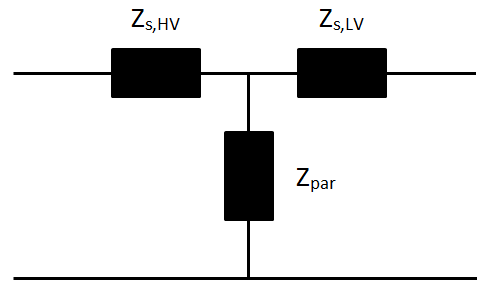
\includegraphics[width=0.65\textwidth, angle=0]{Electric/MyGraphics/trafo_equischeme.png}}
%\caption{Equivalent scheme of a transformer}
%\label{figTrafo}
%\end{figure}

The parallel element ($Z_{par}$) is defined during a no-load test of the transformer. At the primary side, the nominal voltage is applied, while the secondary windings are open. The series elements can be neglected:
\begin{equation}
Z_{par} = \left[ \frac{400}{\sqrt{3}} \right]^2 \left[ \frac{P_0}{3} \right]^{-1}
\label{3Ploss}
\end{equation}
with $P_0$ the no-load losses.

The series elements ($Z_{s,HV}$ and $Z_{s,LV}$) are defined during short-circuit tests of the transformer. During this test, the secondary windings are shorted. Since the parallel elements are large compared to the series elements, the series elements ($Z_s = Z_{s,HV} + Z_{s,LV}$)  can be defined:
\begin{equation}
Z_s = \left[ \frac{400 u_k}{100 \sqrt{3}} \right]^2 \left[ \frac{S_n u_k}{300} \right]^{-1}
\label{3Ploss}
\end{equation}
with $S_n$ the nominal apparent power of the transformer and $u_k$ the percentage of the short-circuit voltage\footnote{The short-circuit voltage is the voltage that has to be applied at the primary winding to have the nominal current in the primary winding when the secondary winding is shorted.}. Generally, $Z_s$ is evenly distributed amongst $Z_{s,HV}$ and $Z_{s,LV}$.

The active losses in a transformer are calculated as is done in Eq.~(\ref{Ploss}) for the losses in the grid. 

\subsection{Photovoltaic generation}

\subsubsection{Photovoltaic panel' power output}

The general current-voltage ($\tv{i}\tim,\tv{u}\tim$) equation for the single diode equivalent circuit is given by \\*
\begin{equation}
\tv{i}\tim = I_{ph} - I_{0} \left(\exp \frac{\tv{u}\tim + \tv{i}\tim R_{s}}{a} - 1 \right) - \frac{\tv{u}\tim + \tv{i}\tim R_{s}}{R_{sh}} \label{eq1}
\end{equation}
which can be used to determine the power output $\tv{P}\tim$ equal to $\tv{i}\tim \tv{v}\tim$ and which can be written for three points, \ie for the short-circuit, the open-circuit and the maximum power point\citep{sera}. The five required parameters are the light current $I_{ph}$, the diode reverse saturation current $I_{0}$, the series resistance $R_{s}$, the shunt resistance $R_{sh}$ and the ideality factor $a$ which depend on the cell temperature $T_{c}$, the total solar irradiation $E_{e}$ and the solar incidence angle $\xi$. \\*
%
The reverse saturation current $I_{o}$ and light current $I_{ph}$ at standard testing conditions can be found based on Eq.~(\ref{eq1}) for the short circuit (Eq.~(\ref{eq4})) and open circuit condition (Eq.~(\ref{eq5})).\\*
\begin{gather}
i_{sc} = I_{ph,\star} - I_{0,\star} \exp \frac{i_{sc} R_{s,\star}}{a_{\star}} - \frac{i_{sc} R_{s,\star}}{R_{sh,\star}} \label{eq4} \\
i_{oc} \triangleq 0 = I_{ph,\star} - I_{0,\star} \exp \frac{u_{oc}}{a_{\star}} - 
\frac{u_{oc}}{R_{sh,\star}}  \label{eq5} \\
i_{mp} = I_{ph,\star} - I_{0,\star} \left(\exp \frac{u_{mp} + i_{mp} R_{s,\star}}{a_{\star}} - 1 \right) - \frac{u_{mp} + i_{mp} R_{s,\star}}{R_{sh,\star}} \label{eq6}
\end{gather}
knowing that $(\mbox{d}ui / \mbox{d}u)\vert_{mp} = 0$ and $(\mbox{d}i / \mbox{d}u)\vert_{sc} = - R_{sh,\star}^{-1}$ \\*
%
The ideality factor has to be corrected for the cell temperature\\*
\begin{equation}
T_{c,\star} \tv{a}\tim = a_{\star} \T_{c} 
\end{equation}

The effective reverse saturation current $\tv{I}_{o}\tim$ can be derived by correcting $I_{0,\star}$ for the cell temperature $\T_{c}$ as\\*
\begin{equation}
T_{c,\star}^{3} \tv{I}_{o}\tim = I_{0,\star} \exp \left( \frac{\epsilon N}{a_{\star}}  \left(1-\frac{T_{c,\star}}{\T_{c}} \right) \right) \T_{c}^{3} 
\end{equation}

The effective light current $\tv{I}_{ph}$ can be derived by correcting $I_{ph,\star}$ for the effective irradiance $\tv{E}_{ef}^{k}$ and the cell temperature $\T_{c}$ as\\*
\begin{gather}
M_{ef,\star} E_{ef,\star} \tv{I}_{ph} = \tv{M}_{ef} \tv{E}_{ef}^{k} \left( I_{ph,\star} + \alpha_{I,sc} \left(\tv{T}_{c} - T_{c,\star}\right) \right) \\
\tv{E}_{ef}^{k} = \left( \tv{\tau}_{\xi,D} \tv{E}_{D}^{k} + \tv{\tau}_{\xi,d} \tv{E}_{d}^{k} \right) \tau_{0}^{-1} \\
\tv{\tau}_{\xi} =  \exp \frac{-f_{k} f_{l}}{\cos \tv{\xi}_{r}} \left(1 - 0.5 \frac{\sin^{2}\tv{\xi}_{r} - \tv{\xi}}{\sin^{2}\tv{\xi}_{r} + \tv{\xi}} + 0.5 \frac{\tan^{2}\tv{\xi}_{r} - \tv{\xi}}{\tan^{2}\tv{\xi}_{r} + \tv{\xi}}  \right) \label{eq7}
\end{gather}

The photovoltaic parameters are adjusted to take into account the position of the sun, the direct and indirect radiation and the ambient temperature. The cell temperature has been adjusted to be the ambient temperature plus the losses of the panel. The parameters for the non-reference conditions are calculated in the next paragraphs.\\*
%
The tilt angle and orientation of the photovoltaic panels are parameters of the PV model. Together with the sun's position, the incidence angle of the direct beam radiation can be calculated which allows to obtain the amount of radiation that gets reflected by and passes through the photovoltaic panel cover. This is done using incidence angle modifiers that are derived from De Soto et al.~\cite{desoto}. The incidence angle modifier $K_{\tau \alpha}(\xi)$ can be found from the transmittance $\tau$ of the cover system with Eq.~(\ref{eq8}), which is approximated in Eq.~(\ref{eq7}). The angle of refraction, $\theta _{r}$, is determined in Eq.~(\ref{eq6}) by Snell's law, with $\xi$ the incidence angle and $n$ the effective index of refraction of the cell cover. In Eq.~(\ref{eq7}), $f_k$ is the glazing extinction coefficient and $f_l$ is the glazing thickness. 

\subsubsection{Power output of photovoltaic system}
A photovoltaic system consists of multiple photovoltaic panels connected in series. Assuming that all photovoltaic panels are in the same condition, the output DC voltage can be multiplied by the number of photovoltaic panels in a photovoltaic system.

The number of photovoltaic panels is a parameter of the general photovoltaic system model. The peak power $P_{mp}$ is defined with $V_{mp}$, $I_{mp}$ and the number of panels $n_p$: \\*
\begin{equation}
\tv{P}_{mp} = n_p \tv{u}_{mp} \tv{i}_{mp}
\label{Ppeak}
\end{equation}

\subsubsection{Inverter}

A photovoltaic system is connected to the electrical grid through an inverter, which converts the generated DC power to AC power with an efficiency $\eta_{dc/ac}$. \\*
%
Due to the lack of simultaneity of production and consumption, a bidirectional energy flow may occur between a building and the electrical grid (\eg low voltage grid for residential buildings), which may lead to voltage instabilities on the grid (\eg increasing voltages due to the injection of electricity, unbalance, etc.). To avoid excessive feeder voltages at the moments of re-injecting photovoltaic power in the grid, the inverter is curtailed when a predefined voltage limit is reached. Curtailing of a photovoltaic system means production losses.


\section{Electrical in-home grid}
In progress.

\section{Electrical storage}
In progress.